\section{Introducción}
\label{sec:introducción}

\par \textbf{SidelabCode Stack} es una forja de desarrollo de Software para su uso como herramienta \textbf{ALM}. Es una herramienta FLOSS (Free Libre Open Source Software) con Licencia \textbf{TBC}.

\begin{figure}[h]
    \begin{center}	
        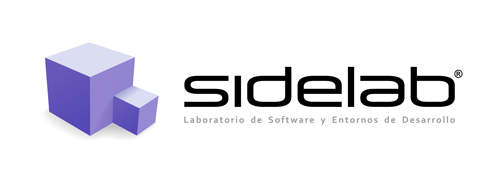
\includegraphics[width=1\textwidth]{sidelab}
        \label{fig:sidelab}
    \end{center}
\end{figure}

\par El desarrollo de este proyecto se basa en el diseño e implementación de la forja SidelabCode Stack ahondando en la definición de un proceso de desarrollo de Software para el diseño de la forja, unificando herramientas a través de la interoperabilidad y facilitando la instalación, la replicación y la recuperación de los datos mediante el uso de Software Libre para construir Software de calidad.

\subsection{Etimología}
\label{sub:etimologia}

\par Sidelab es, un laboratorio de software. Partiendo de esta base, encontramos una definición exacta para SidelabCode \footnote{\url{http://code.sidelab.es/projects/sidelab/wiki/Sidelab}}:

\begin{quotation}
        \emph{Sidelab es el "laboratorio de software y entornos de desarrollo integrados" (Software and Integrated Development Environments Laboratory). Es un grupo de entusiastas de la programación con interés en prácticamente todos los aspectos del desarollo, desde los lenguajes de programación y los algoritmos avanzados, hasta la ingeniería del software y la seguridad informática. Nuestros principales intereses se centran en el desarrollo software y la mejora y personalización de los entornos de desarrollo integrados (IDEs) y herramientas relacionadas.}
\end{quotation}

\par En el caso de Code se refiere al código en sí hacia donde se orienta esta herramienta y Stack, es una pila de servicios para la gestión y el desarrollo de proyectos software.

\par Como resultado tenemos \textbf{SidelabCode Stack} una Forja de desarrollo de aplicaciones.

% subsection etimologia (end)